%%%%%%%%%%%%%%%%%%%%%%%%%%%%%%%%%%%%%%%%%%%%%%%%%%%%%%%%%% 
\chapter{クイーン支配問題}\label{chap:background}
%%%%%%%%%%%%%%%%%%%%%%%%%%%%%%%%%%%%%%%%%%%%%%%%%%%%%%%%%% 

\section{支配集合問題}
グラフ$G=(V,E)$の頂点の部分集合$S\subset V$と
その隣接頂点の集合との和集合が$V$と一致するとき,
$S$を$G$の\textbf{支配集合}という.
支配集合$S$の要素数を\textbf{サイズ}という.
 \begin{itemize}
  \item サイズが最小の支配集合を\textbf{最小支配集合}という.
  \item 最小支配集合のサイズをグラフ$G$の\textbf{支配数}と呼ぶ.
    本論文ではグラフ$G$の支配数を$\gamma(G)$で表す.
 \end{itemize}

グラフ$G$と正の整数$k$が与えられたとき,
サイズが$k$の$G$の支配集合が存在するかどうかを
判定する問題を\textbf{支配集合問題}という.
支配集合問題は\textbf{NP完全}に属する問題であることが証明されている~\cite{Jhonson79}.

\section{クイーン支配問題}
$n\times n$のチェス盤について各マスを頂点とし,
クイーンが移動できるマス同士が辺で結ばれているグラフを
\textbf{クイーングラフ}という.
サイズ$n\times n$のクイーングラフを$Q_n$で表す.
例えば,サイズ3のチェス盤とクイーングラフ$Q_3$の対応関係は
図~\ref{ex:queengraph_3}のようになる.

クイーングラフ$Q_n$と正の整数$k$が与えられたとき,
サイズ$k$の$Q_n$の支配集合が存在するかどうか判定する問題を
\textbf{クイーン支配問題}という. \par
クイーングラフの支配数は,1862年に~\cite{Jaenisch62}で$\gamma(Q_8)=5$が示されてから研究されており,$n=3,11$を除いて$n \leq 132$で$\lceil n/2 \rceil \leq \gamma(Q_n) \leq \lceil n/2 \rceil +1 $であることが証明されている~\cite{Ostergard01}.

表\ref{tb:queen_n}にクイーングラフ$Q_n$に対する支配数$\gamma(Q_n)$の上下限を示した.



図\ref{ex:queengraph5}は,$Q_5$の最小支配集合の例である.
3個のクイーンを置いたとき,
クイーンを移動させて全てのマスにアタック可能である.
また,2個または1個のクイーンを置いたとき,
クイーンを移動させて全てのマスにアタックすることは不可能である.

 \begin{figure}[htb]
   \centering
   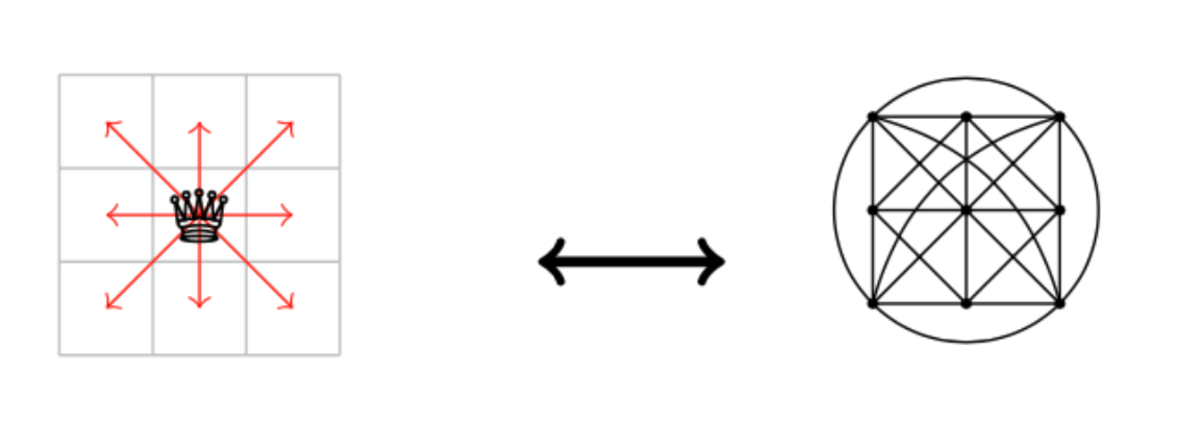
\includegraphics[width=1.0\linewidth]{fig/fig-queen_3_graph.pdf}
   \caption{$3 \times 3$のチェス盤とクイーングラフ$Q_3$の対応関係}
   \label{ex:queengraph_3}
 \end{figure}

\begin{table}[hbtp]
   \centering
   \caption{$n$と$\gamma(Q_n)$の上下限}
   \begin{tabular}{c|c||c|c||c|c||c|c||c|c} \hline
    $n$ & $\gamma(Q_{n})$ & $n$ & $\gamma(Q_{n})$ &$n$ & $\gamma(Q_{n})$ &$n$ & $\gamma(Q_{n})$ \\ \hline \hline
    1 &1 &6 &3 &11 &5 &16 &9 &21 &11\\ \hline
    2 &1 &7 &4 &12 &6 &17 &9 &22 &11-12\\ \hline
    3 &1 &8 &5 &13 &7 &18 &9 &23 &12\\ \hline
    4 &2 &9 &5 &14 &8 &19 &10 &24 &12-13\\ \hline
    5 &3 &10 &5 &15 &9 &20 &11 &25 &13\\ \hline
   \end{tabular}
   \label{tb:queen_n}
  \end{table}


\begin{figure}[htb]
  \centering
  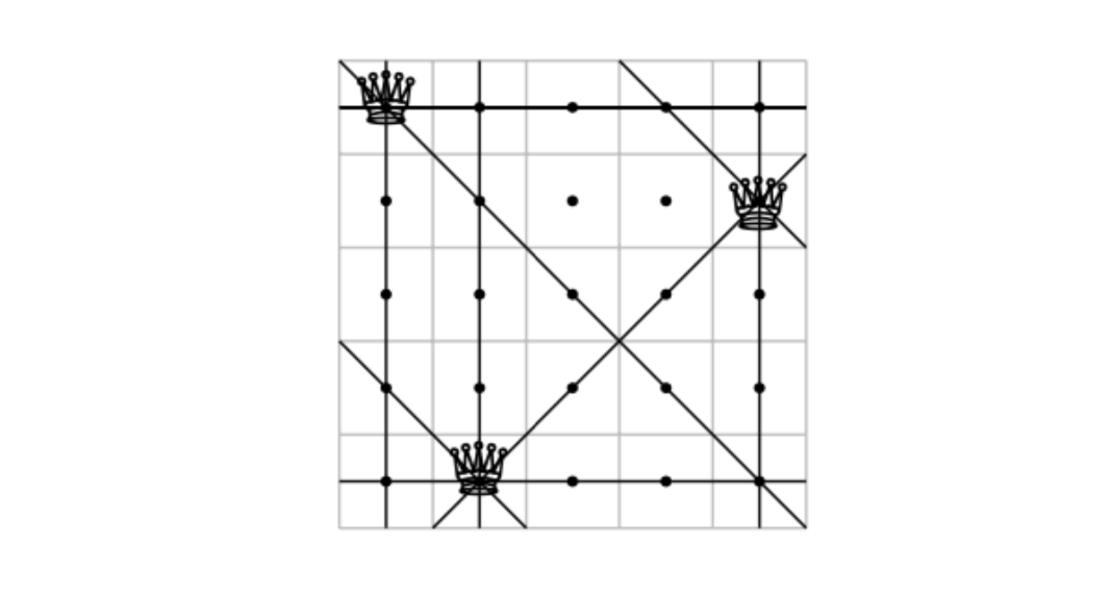
\includegraphics[width=0.6 \linewidth]{fig/fig-queen_5.pdf}
  \caption{$Q_5$の最小支配集合の例}
  \label{ex:queengraph5}
\end{figure}

%%% Local Variables:
%%% mode: latex
%%% TeX-master: "paper"
%%% End:
